\chapter{Problématique}
\section{Introduction}

Dans ce chapitre, nous allons 
\newpage 
\section{Contexte}
\subsection{Histoire de l'apprentissage approfondie}
Cette section est basée sur l'article de Tim Dettmers \cite{DeepLearningHistory}
\subsubsection{Réseaux de Neurones}
L'origine des réseaux de neurones, peut être considéré de Ivakhnenko et Lapa \cite{FirstDeepNN} qui ont réussi à implémenter un réseau neuronale à fonctions d'activations polynomiales. Mais ils n'ont pas utilisé la propagation en arrière qui n'était pas répandues dans ces années.
\subsubsection{Propfagation en Arrière} 
La propagation en arrière était dérivée dans les années 1960 mais sous une forme incomplète et inefficace. En outre, sa forme moderne était dérivée par Linnainmaa dans sa thèse de mastère \cite{OriginalBackPropagation} "Taylor expansion of the accumulated rounding error" en 1970. La propagation ne serait répandues que dans 1985 dans lequel les recherches on montré qu'elle donne des répresentations interréssantes des paramètres.
\subsubsection{L'hiver de l'IA}
Malgrès les succès de la propagation en arrière, et son incorporation dans les couches convolutionnelles (LeNet \cite{LeNet}) et récurrentes (spécifiquement LSTM \cite{LSTMPaper}), l'intérêt à l'intelligence artificielle était minimale dans les années 1980-1990, et les avancement dans ce domaine étaient minimales.
\newline De plus, les machines à vecteurs de supports (SVM \cite{OriginalSVM}) étaient préférés au lieu des réseaux de neurones vu la complexité de ces derniers.
\subsubsection{Réapparition grâce aux GPUs}
Grâce au progrès des ordinateurs, et l'arrivée des cartes graphiques (GPUs), l'utilisation des réseaux de neurones était de plus en plus pratique, et progressivement, la complexité de ces réseaux croît.
\subsubsection{Explosion de l'apprentissage approfondie}
Le moment décisif à l'apprentissage approfondie était le succès de Krizhevsky, Sutskever et Hinton \cite{NIPS2012_c399862d} à créer un réseau de neurones profonds avec lequel ils on importé la compétition de ILSVRC-2012 ImageNet.
\newline Ce moment a marqué l'abandon l'ingénierie des fonctionnalités et le début de l'apprentissage des fonctionnalités. Et puis, Facebook, Google et Microsoft ont rapidement investi dans la recherche de l'apprentissage approfondie.
\subsubsection{Un niveau surhumain}
Dès les années 2010s, beaucoup de modèles de IA ont montré un niveau surhumain dans des tâches que nous avons cru impénetrable par les ordinateurs.
\newline Comme un exemple pertinant, nous allons parler de la suite Alpha dévéloppée par l'équipe DeepMing de Google:
\begin{enumerate}
	\item Le modèle AlphaGo était le premier agent ayant un élo surhumain, ceci est prouvé par son match historique en 2016 contre Lee Sedol\footnote{Lee Sedol est un des joueurs de Go les plus accomplis dans l'histoire du jeu, avec 18 titres internationals. } dans lequel AlphaGo a gagné 4-1 contre lui\footnote{Ce match était une des cause pour laquelle Lee Sedol s'est retiré de Go en 2019. Il a cité que le IA est "une entité qui ne pourrait être vaincue."}.
	\item Le modèle AlphaGo Zero est une amélioration de AlphaGo. La majeure différence est dans son entraînement, qui n'est pas basé sur des jeux entre des humains comme le cas de AlphaGo, mais il s'est entraîné en jouant contre lui-même.
	\item Le modèle AlphaZero est encore une amélioration de AlphaGo Zero, qui avait un niveau surhumain dans Go, Shogi et l'échec\footnote{Dans l'échec, il a même écrasé Stockfish en 2018 avec un résultat de (+155 -6 =839). Avant l'apparition de Alpha Zero, Stockfish était le plus puissant moteur d'échec.}
\end{enumerate}
\begin{figure}[h!]
	\centering
	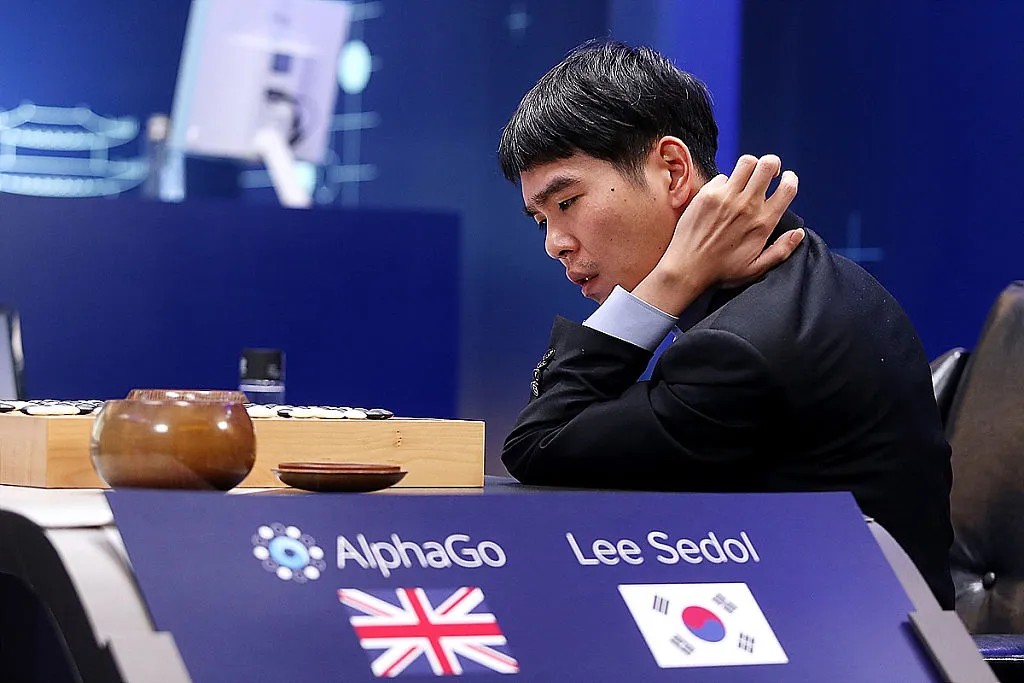
\includegraphics[width=.7\textwidth]{Figures/go-lee-sedol.png}
	\caption{Lee Sedol analysant le tablier après sa première victoire du match}
	\label{fig:LeeSedolVsAlphaGo}
\end{figure}
\FloatBarrier
\subsection{Le coût de l'IA}
Cette explosion de l'IA a causé une explosion dans les coûts de leurs entraînement, déploiement et fonctionnement.


\subsubsection{Le coût économique}
Les modèles d'intelligences artificielles les plus robustes nécessitent des ressources énormes pour leur entraînement et même fonctionnement.
\newline En effet: 
\begin{itemize}
	\item L'entraînement de AlphaGo Zero a coûté approximativement 25 millions de dollars \cite{AlphaGoZeroCost}.
	\item L'entraînement de NAS a coûté approximativement 3 millions de dollars \cite{ShrinkingDeepLearningCarbon}.
\end{itemize}
\subsubsection{Le coût énergitique}
L'utilisation gigantesque des ressources causent une consommation énorme d'énergie.
\newline Par exemple:
\begin{itemize}
	\item Dans le match contre Lee Sedol, AlphaGo a utilisé 1202 GPUs et 176 CPUs. Une estimation de la puissance consommé montre un chiffre colossal de $1$ mégawatts \cite{ShrinkingDeepLearningCarbon}.
	\item Pour entraîner NAS, l'énergie totale consommée est estimée à $656347 \ \text{kWh}$ \cite{CO2Footprint}.
\end{itemize}
\subsubsection{Le coût environmental}
Le coût environmental des modèles IA avancés est souvent très importants. 
\newline En effet, les estimations de $\text{CO}_2$ générés par ces algorithmes peut dépasser l'ordre de milliers de kilogrammes:
\begin{itemize}
	\item 
\end{itemize}
\begin{table}[ht]
	\small
	\centering
	\begin{tabularx}{\textwidth}{| p{3cm} | X | X | p{2cm} | p{2.2cm} | p{3cm} |}
		\hline
		Modèle / Objet & Hardware & Puissance (Watt) & Temps de fonctionnement (Heures) & $\text{CO}_2$ équivalents (kg) & Budget cloud (dollars américains) \\
		\hline 
		Transformer\textsubscript{base} & P100x8 & 1415.78 & 12 & 11.79 & \$41 - \$410 \\
		\hline
		Transformer\textsubscript{big} & P100x8 & 1515.43 & 84 & 87.08 & \$289 - \$981 \\
		\hline
		ELMo & P100x3 & 1415.78 & 12 & 11.79 & \$433 - \$1472 \\
		\hline
		BERT\textsubscript{base} & V100x64 & 12041.51 & 79 & 652.27 & \$3751 - \$12571 \\ 
		\hline
		NAS & P100x8 & 1515.43 & 274120 & 284019 & \$942973 - \$3201722 \\
		\hline
		AlphaGo & & $\approx 1000000$ & 960 & 96000 & $\approx \$250000000$ \\ 
		\hline
		Climatiseur& & 840 &  &  & \\
		\hline
		Refrégirateur & & 1233 & & & \\
		\hline
		Avion SF $\rightarrow$ NY  & & & & 900 & \\
		\hline
		Personne durant 1 an & & & & 5000 & \\
		\hline
		Voiture durant sa vie & & & & 57152 & \\
		\hline
		Maison durant son construction \cite{HouseCarbonFootprint} & & & & 50000 - 80000 &  \\
		\hline
	\end{tabularx}
	\caption{Coût des modèles de IA.}
	\label{table:EnergyConsumption}
	
\end{table}
\FloatBarrier
\subsection{Les limites des systèmes embarqués}
\newpage 
\section{Le Binary Neural Network}
\subsection{Introduction}
\subsection{La signification de "Binary"}
\newpage 
\section{BinaryFlow}
\subsection{Introduction}
BinaryFlow est une bibliothèque de Deep Learning basée sur Larq et TensorFlow
\subsection{Raison d'exister}
\subsection{Signification du nom}
Le choix de nom "BinaryFlow" est influencé de nom "TensorFlow" de la fameuse bibliothèque d'apprentissage automatique et de programmation différentielle qui est crée et maintenue par Google.
\newline TensorFlow se traduit en "flux de tenseurs" qui est l'utilisation excessive  des tenseurs - qui sont grosso modo des tableaux numériques multidimensionnels - dans les calculs différentiels.
\newline Par analogie, BinaryFlow se traduit en "flux binaire" qui signifie l'utilisation excessive des opérations booléennes sur des tenseurs binaires.
\subsection{Solutions offertes par BinaryFlow}
\subsubsection{Couches}
BinaryFlow supporte toutes les couches offertes par TensorFlow et Larq. Mais il aussi supporte:
\begin{itemize}
	\item BinaryNet: Dense, ConvND, TransposedConvND, SeparableConvND.
	\item XnorNet: Dense, ConvND.
	\item XnorNet++: Dense, ConvND.
	\item ABCNet: Dense, Conv1D, Conv2D, Conv3D
	\item BiRealNet: Dense, Conv1D, Conv2D, Conv3D
	\item MeliusNet: Dense, Conv1D, Conv2D, Conv3D
\end{itemize}
\subsubsection{Binarisations}
BinaryFlow supporte toutes les binarisations standard offertes par Larq, et les étend en ajoutant:
\begin{itemize}
	\item Binarisation décalée: qui est une méta-binarisation, qui prend une binarisation $\Psi$ et donne $\Psi_\mu=x\rightarrow \Psi(x+\mu)$ avec $\mu \in\mathbb{R}$ entraînable
	\item Binarisation stochastique: qui est une méta-binaristation qui prend une distribution de probabilité réelle $\mathcal{D}$ en paramètre, et une binarisation $\Psi$, et donne la fonction: $x\rightarrow  \Psi(x-z)$ avec $z\sim U$
	\item Binarisation stochastique décalée
	
\end{itemize}
\subsubsection{Optimiseurs}
BinaryFlow offre les optimiseurs suivants
\begin{itemize}
	\item SGD
	\item Adam\cite{AdamOptimizer}
	\item Bob\cite{BopOptimizer}
\end{itemize}
\subsubsection{Déploiement}
BinaryFlow conserve tous les optimisations offerte par Larq